\documentclass[12pt, oneside, openany]{book}

\usepackage{mathptmx} % Contiene una fuente similar a Times New Roman

\usepackage[spanish, es-tabla]{babel} % Permite escritura en castellano
\usepackage[utf8]{inputenc} % Permite utilizar caracteres UTF8

\usepackage{graphicx} % Para la inclusión de gráficos e imágenes
\graphicspath{ {images/} } % Ruta para buscar las imágenes
\usepackage[a4paper,top=30mm,left=30mm,right=25mm,bottom=25mm,headheight=20mm]{geometry} % Configuración de los margenes de la página

% Paquetes para que funcione el formato.
\usepackage{titlesec}
\usepackage{setspace}
\usepackage{ragged2e}
\usepackage{fancyhdr}
\usepackage{lastpage}
\usepackage{listings}
\usepackage{stackengine}
\usepackage{array}
\usepackage[hidelinks]{hyperref}
\usepackage{enumitem}
\usepackage{float}
\usepackage{upquote}
\usepackage{hypcap}
\usepackage{caption}
\usepackage{fancyvrb}
\usepackage{hyperref} % Paquete para que las referencias funcionen, y permite introducir links
\usepackage{xcolor} % Paquete para trabajar con colores (fondo de celdas, color del texto...)

% Se define un color gris desde su código RGB
\definecolor{gris}{RGB}{220,220,220}

\setcounter{secnumdepth}{3} % Para permitir numerar las sub-subsecciones

% Modifica el nombre de los índices al castellano
\addto\captionsspanish{
  \renewcommand{\contentsname}{Índice de contenido}
  \renewcommand{\listfigurename}{Índice de figuras}
  \renewcommand{\listtablename}{Índice de tablas}
}

% Formateo de los nombres de los apartados:
\titleformat{\chapter}[block]
  {\normalfont\Huge\bfseries\singlespacing}{\thechapter.}{1em}{\Huge}
\titlespacing*{\chapter}{0pt}{-62pt}{0pt}

\titleformat{\section}[block]
  {\normalfont\Large\bfseries}{\thesection.}{4pt}{\Large}
\titlespacing*{\section}{0pt}{\baselineskip}{0pt}

\titleformat{\subsection}[block]
  {\normalfont\large\bfseries}{\thesubsection.}{4pt}{\normalsize\large}
\titlespacing*{\subsection}{0pt}{0pt}{0pt}

\titleformat{\subsubsection}[block]
  {\normalfont\normalsize\bfseries}{\thesubsubsection.}{4pt}{\normalsize}
\titlespacing*{\subsubsection}{0pt}{0pt}{0pt}

\def\tablename{Tabla}

%% Variables para portada y cabeceras
%% Cambiar los valores para cada documento!!!
\def\title{Memoria de Prácticas}
\def\subject{Ingeniería de Servicios}
\def\authorOne{Juan Francisco Mier Montoto}
\def\authorOneId{UO283319}
\def\authorTwo{Alejandro Rodríguez López}
\def\authorTwoId{UO281827}
\def\group{PL 3,~grupo 1}
\def\date{enero 2024}
\def\org{Escuela Politécnica de Ingeniería de Gijón}
\def\area{Grado en Ingeniería Informática en Tecnologías de la Información}

\def\ORG{\expandafter\MakeUppercase\expandafter{\org}}
\def\AREA{\expandafter\MakeUppercase\expandafter{\area}}
\def\SUBJECT{\expandafter\MakeUppercase\expandafter{\subject}}
\def\authors{\authorOne{,}~\authorTwo}

\captionsetup{justification=centering}
\setlength{\headheight}{65pt}

\fancyhf{}
\fancyhead[L]{
\includegraphics[height=16mm]{style/square.png}
  \hspace{1em} \Longstack[l] {
    \textbf{\SUBJECT} \newline
    \textbf{\title}}
  \newline \leftmark{}
}
\fancyhead[R]{\bfseries{Hoja \hyperlink{toc}{\thepage}~de~\pageref{LastPage}}}
\fancyfoot[C]{\authors}
\renewcommand{\headrulewidth}{0pt} % default is 0pt
\renewcommand{\footrulewidth}{0.4pt} % default is 0

\fancypagestyle{plain}{%
  \fancyhf{}
  \fancyhead[L]{
\includegraphics[height=16mm]{style/square.png}
    \hspace{1em} \Longstack[l]{
      \textbf{\SUBJECT} \newline
      \textbf{\title}}}
  \fancyhead[R]{\bfseries{Hoja \hyperlink{toc}{\thepage}~de~\pageref{LastPage}}}
  \fancyfoot[C]{\authors}
  \renewcommand{\headrulewidth}{0pt} % default is 0pt
  \renewcommand{\footrulewidth}{0.4pt} % default is 0pt
}

\pagestyle{fancy}

\restylefloat{table}


\begin{document}

\rmfamily % Fuente tipo Romana

% Portada de la memoria
\begin{titlepage}
    \centering
    \bfseries {
        \null{}
        \vspace{0cm}
        \begin{table}[h]
            \centering
            \begin{tabular}{m{10cm} m{1cm} m{3cm}}
                \vspace{0.2cm}
                
\includegraphics[width=86mm]{style/full.png} &  & \vspace{1.52mm} 
\includegraphics[width=23mm]{style/square.png} \\
            \end{tabular}
        \end{table}

        \vspace{3\baselineskip}

        \Large{\ORG{} \\ \vspace{3\baselineskip}}
        \large {
            \AREA{} \\ \vspace{3\baselineskip}
            \subject{} \\ \vspace{2\baselineskip}

            % TRABAJO FIN DE GRADO/MÁSTER Nº XXXXXXXXX \vspace{\baselineskip} \\
            \title{} \\ \vspace{3\baselineskip}

            \author{} \\
            \authorid{} \\
            % TUTOR/ES: \\
            % D. APELLIDO1 APELLIDO2, Nombre \\
            % D. APELLIDO1 APELLIDO2, Nombre \\  \vspace{\baselineskip}

            \vspace{2\baselineskip}
            FECHA:\@ \date{}
        }
    }
\end{titlepage}


% Índice de contenido
\addcontentsline{toc}{chapter}{Índice de contenido} % Añade la referencia al índice de contenido
\hypertarget{toc}{}
\tableofcontents
\newpage{}

% Índice de figuras
\addcontentsline{toc}{chapter}{Índice de figuras}  % Añade la referencia al índice de contenido
\hypertarget{lof}{}
\listoffigures

\justify{} % Texto justificado
\setlength{\parskip}{\baselineskip} % Separación entre párrafos de 1 linea
\onehalfspacing{}

%% El contenido de la memoria, dividido en capítulos:
\Chapter{Servicios básicos}{UDP y TCP}
\section{Programación de red: UDP}
\subsection{Módulos de ayuda}
Para esta práctica, se desarrollan módulos de Python que faciliten las tareas básicas,
como lecturas de hosts y puertos por argumentos: \\
\begin{minipage}{\linewidth}
	\centering
	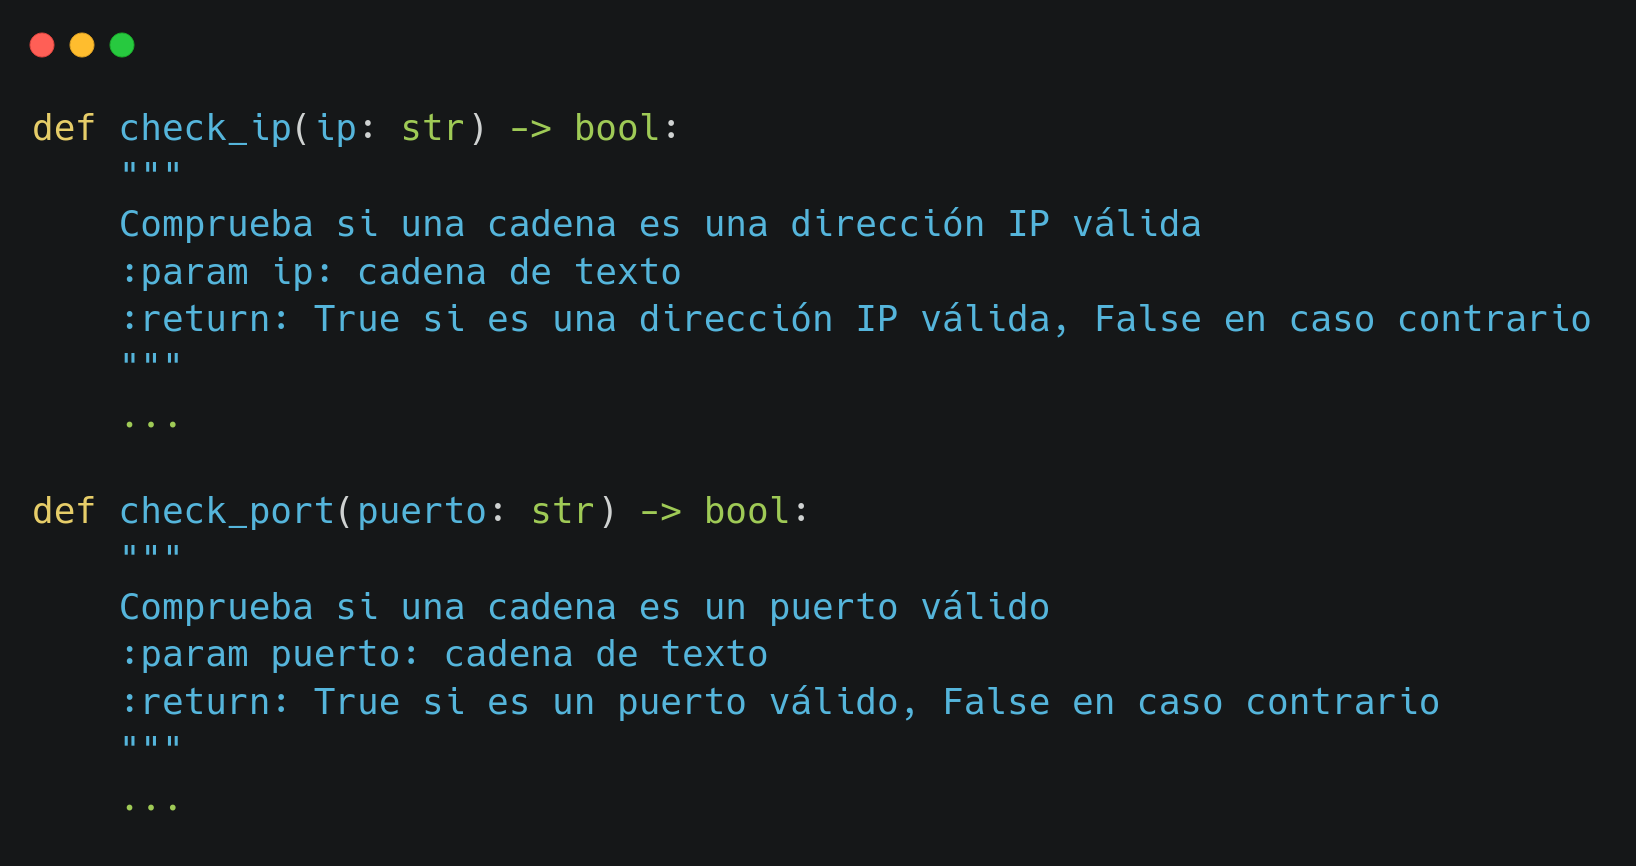
\includegraphics[width=1\textwidth]{1/code1.png}
	\captionof{figure}{Estructura del módulo de ayuda ``ips.py''}\label{fig:1/code1}
\end{minipage}
\\
\begin{minipage}{\linewidth}
	\centering
	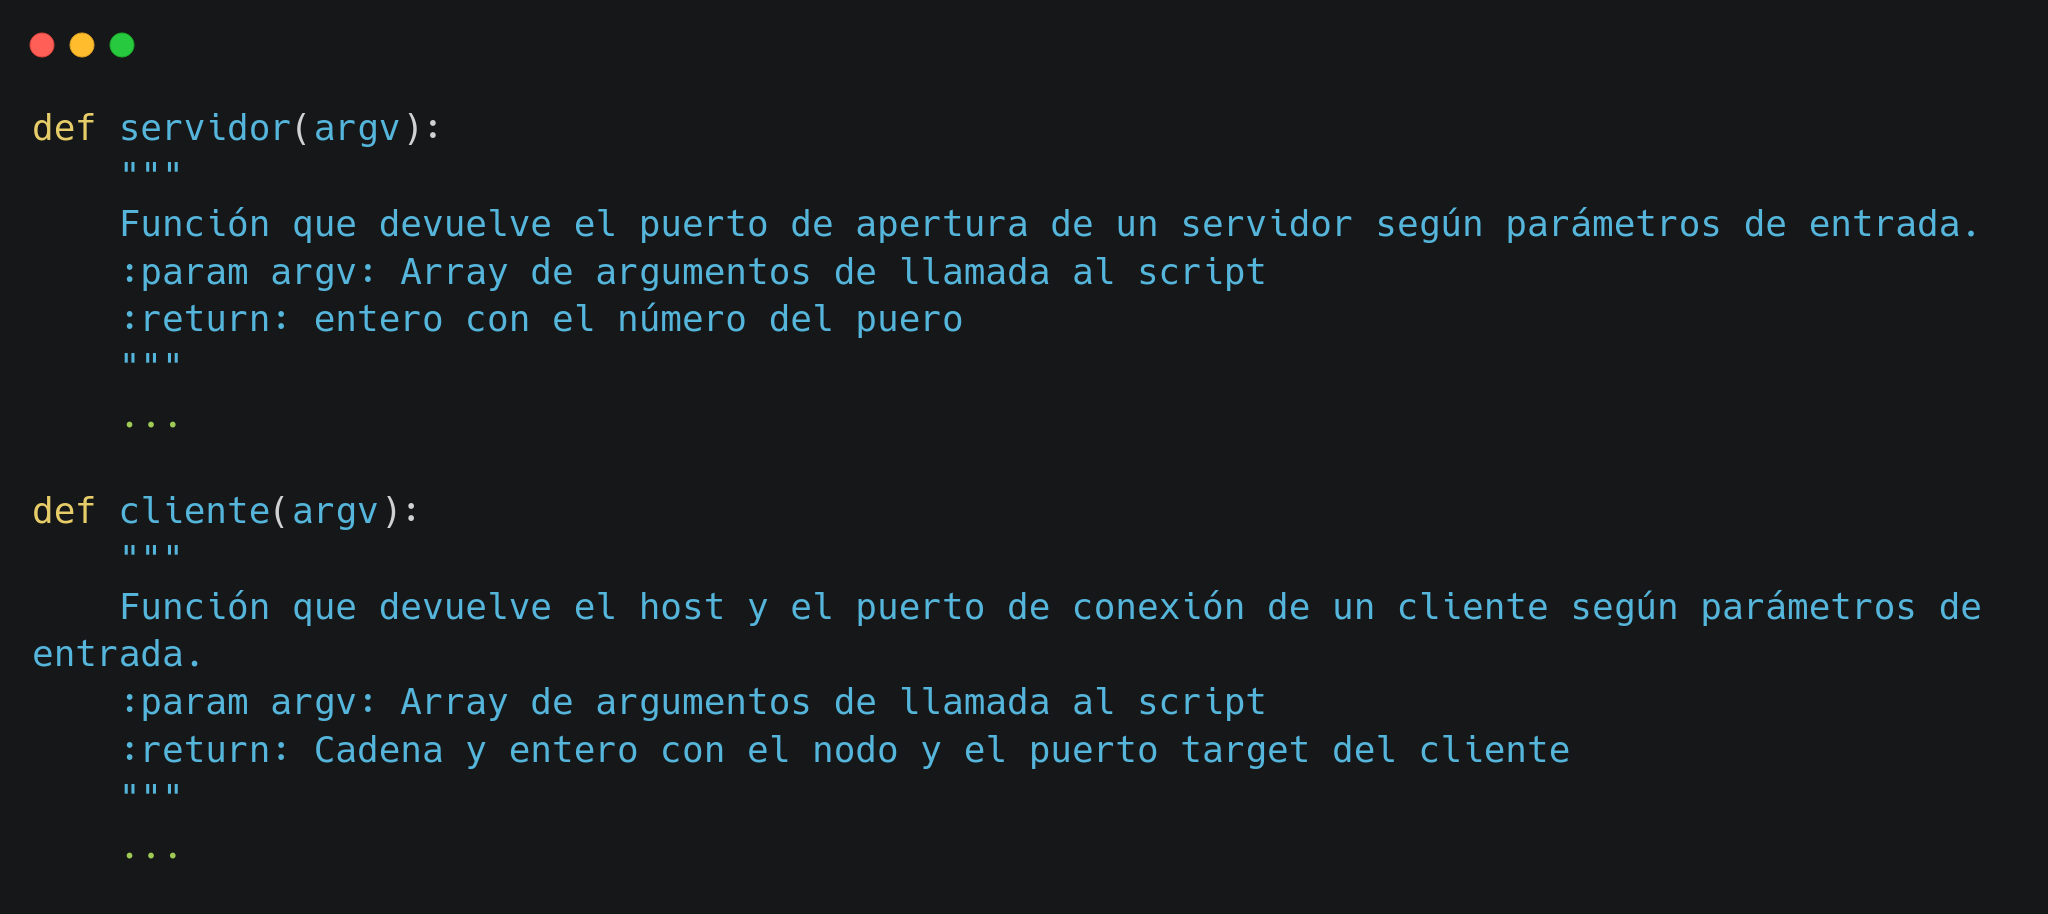
\includegraphics[width=1\textwidth]{1/code2.png}
	\captionof{figure}{Estructura del módulo de ayuda ``ips\_argv.py''}\label{fig:1/code2}
\end{minipage}

\subsection{Ejercicio 1}

\subsection{Ejercicio 2}

\subsection{Ejercicio 3}

\subsection{Ejercicio 4}

\section{Programación de red: TCP}
\subsection{Módulos de ayuda}
Se reutilizan los módulos de la sesión anterior (\ref{fig:1/code1}~y~\ref{fig:1/code2}) para
realizar todos los ejercicios. Además, para los ejercicios ``oche'' se reutiliza el código
usando otro módulo nuevo: \\
\begin{minipage}{\linewidth}
	\centering
	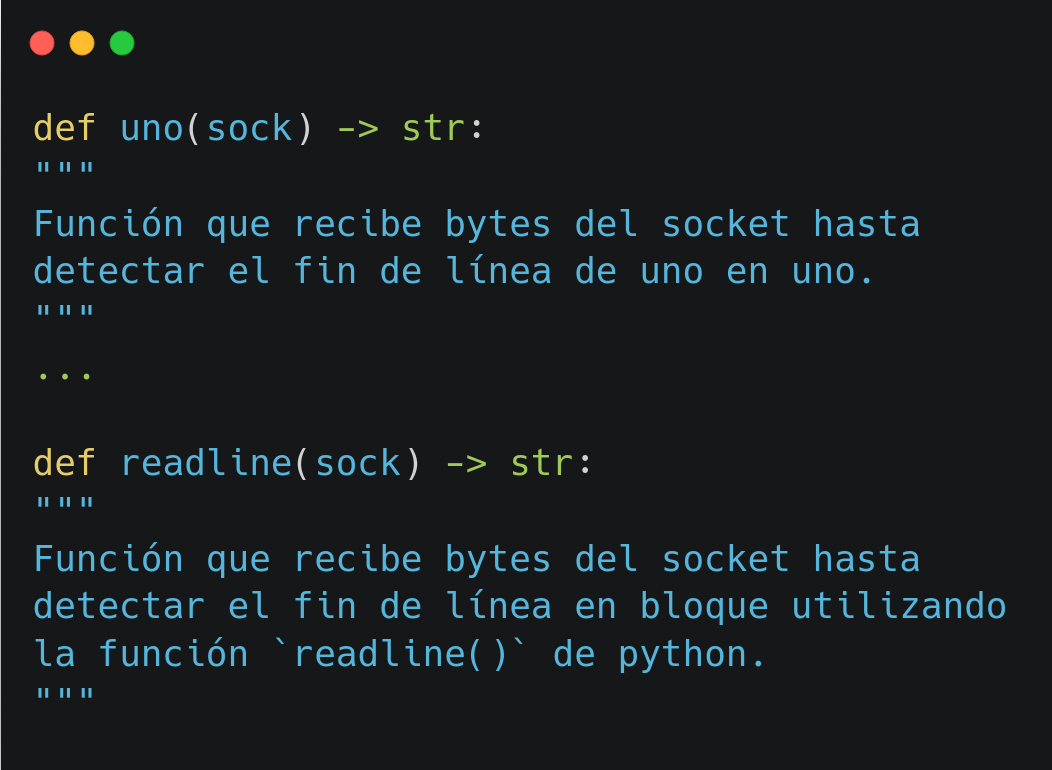
\includegraphics[width=1\textwidth]{1/code3.png}
	\captionof{figure}{Estructura del módulo de ayuda ``recibir\_mensaje.py''}\label{fig:1/code3}
\end{minipage}

\subsection{Ejercicio 1}

\subsection{Ejercicio 2}

\subsection{Experimento}

\subsection{Ejercicio 3 / Experimento}

\subsection{Ejercicio 4 / Experimento}

\subsection{Ejercicio 5}

\subsection{Ejercicio 6}

\subsection{Ejercicio 7 (opcional)}

\subsection{Experimento + Ejercicio Docker}

\Chapter{Servicios web}{Infraestructura y Aplicaciones}
\section{Instalación de infraestructura web}

\section{Aplicaciones web y HTTP}

\chapter{Acceso remoto y transferencia}\label{chap:3}
Esta práctica se centra en protocolos muy utilizados en la actualidad para
acceder a máquinas remotas y transferir archivos entre ellas. No se ha
realizado el apartado opcional de FTP{.}

Todo el código de esta práctica se encuentra dividido en carpetas según
el protocolo sobre el que se está trabajando. En cada carpeta se encuentran
los ficheros de cada ejercicio, con el nombre del ejercicio en cuestión.

\section{Acceso remoto}
\subsection{Telnet}
Para la realización de este apartado, se instala el servidor \Verb#telnetd# y su cliente y
se activa.

\begin{minipage}{\linewidth}
    \centering
    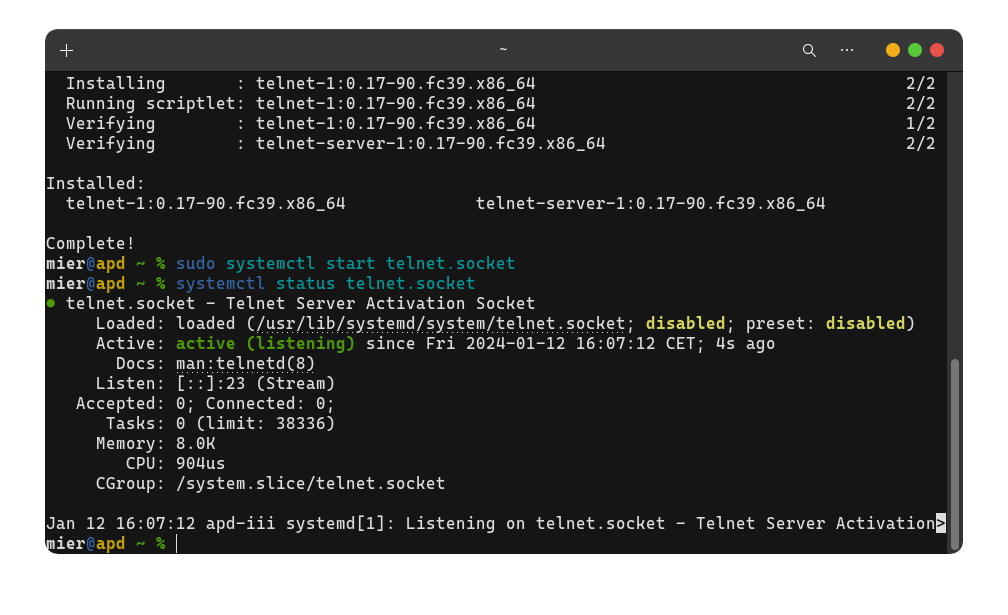
\includegraphics[width=\textwidth]{3/telnet0.png}
    \captionof{figure}{Instalación del servidor Telnet}\label{fig:3/1}
\end{minipage}

Como recuerda el enunciado, el servidor telnet no es seguro, por lo que se ha de desactivar
tras el desarrollo de los ejercicios.

Los siguientes ejercicios son solo pequeñas demostraciones prácticas sobre el protocolo, por
lo que no tienen grandes explicaciones.

\subsubsection{Ejercicio 1}
El ejercicio solicita que se escriba un programa \lstinline{telnet1_ejemplo.py}
que muestre por pantalla el resultado de ejecutar la orden \lstinline{ls} en el
directorio \Verb#/home#.

\begin{minipage}{\linewidth}
    \centering
    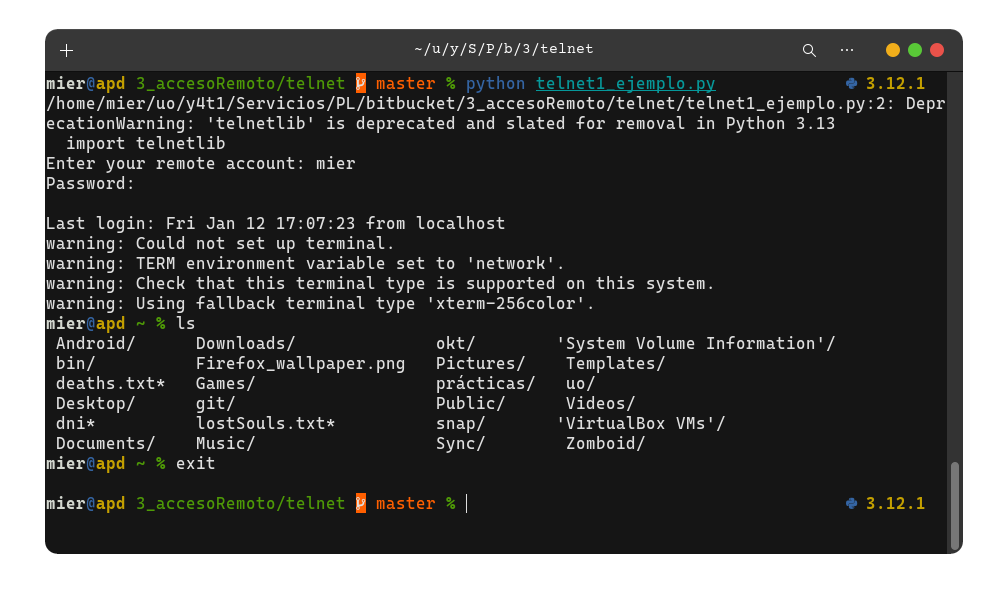
\includegraphics[width=\textwidth]{3/telnet1.png}
    \captionof{figure}{Ejercicio de ejemplo de Telnet}\label{fig:3/2}
\end{minipage}

El ejercicio solicita posteriormente que se mejore el programa \\
(\Verb#telnet1_ejemplo_mejorado.py#) para que omita el mensaje de bienvenida
del sistema.

\begin{minipage}{\linewidth}
    \centering
    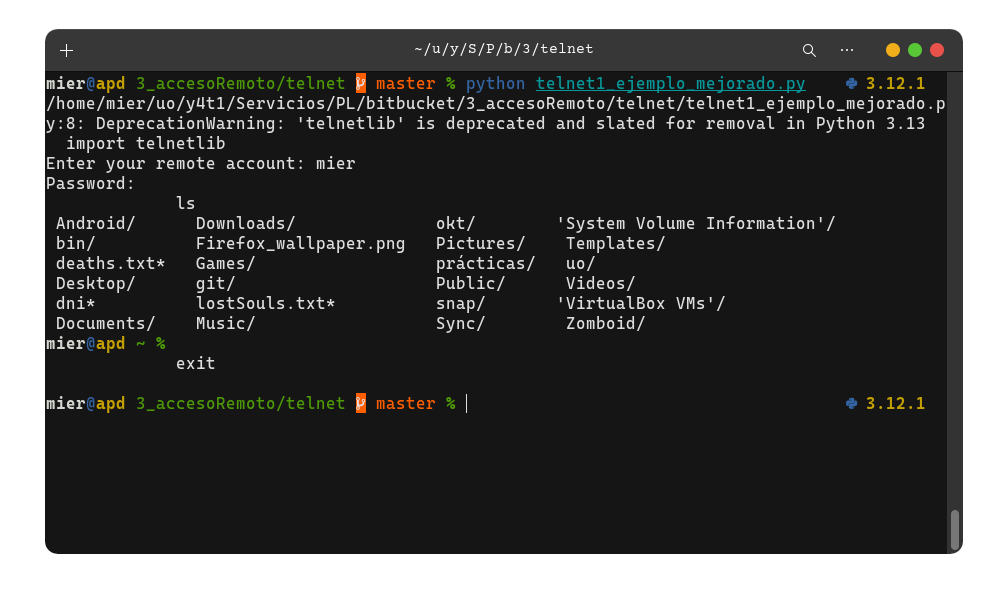
\includegraphics[width=\textwidth]{3/telnet2.png}
    \captionof{figure}{Ejercicio de ejemplo de Telnet mejorado}\label{fig:3/3}
\end{minipage}

\subsubsection{Ejercicio 2}

El ejercicio solicita escribir un programa \Verb#telnet2_lanza_servidor.py#
que lance un programa de la sesión \nameref{chap:1}.

Debido a que esta práctica se realiza en una máquina física Linux donde se acortan
los nombres de los procesos que se envían a través del comando \Verb#ps -ef#, el
ejercicio no funciona como esperado. El código que no funciona (validado por el
profesor) es el siguiente:

\begin{minipage}{\linewidth}
    \centering
    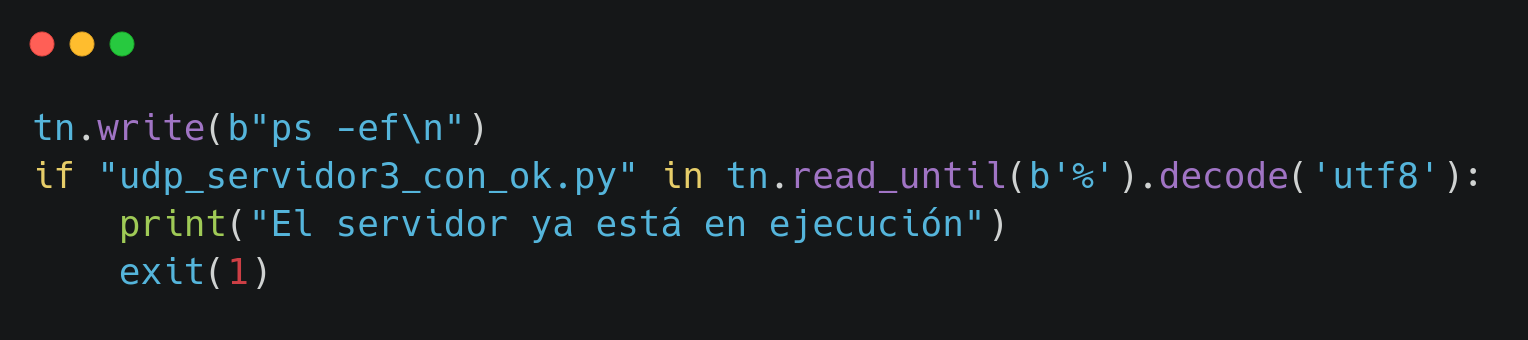
\includegraphics[width=\textwidth]{3/telnet_code1.png}
    \captionof{figure}{Código del ejercicio 2}\label{fig:3/4}
\end{minipage}

De todas formas, la esencia de la práctica es utilizar telnet para lanzar el servidor
UDP, por lo que se ignora la parte de la comprobación de procesos.

\begin{minipage}{\linewidth}
    \centering
    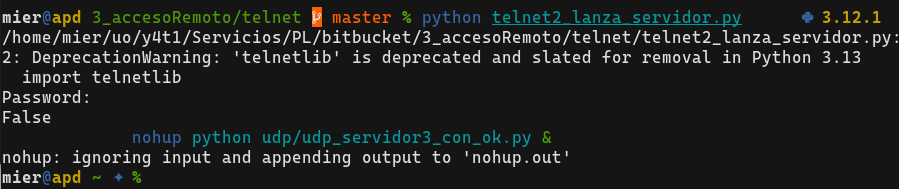
\includegraphics[width=\textwidth]{3/telnet3.png}
    \captionof{figure}{Telnet lanzando servidor UDP a través de nohup}\label{fig:3/5}
\end{minipage}

\subsection{SSH}
Puesto que el servidor SSH ya se encuentra instalado en la máquina, no es necesario
instalarlo. Todas las prácticas se realizan en plataformas Linux, por lo que se
utilizan las contrapartes de los programas de Windows que se utilizan en el enunciado.

\subsubsection{Ejercicio 3}
En este ejercicio, en lugar de PuTTY se utiliza el comand \Verb#ssh# directamente
para conectarse a un servidor remoto y verificar las huellas.

Para realizar este ejercicio, se utiliza un servidor externo que tenga SSH activado
y que nos permita obtener toda la información necesaria.

Al ejecutar el comando que nos otorga el fingerprint de la clave ED25519, obtenemos
el siguiente resultado: \Verb#SHA256:XWZjJrS...#. Al tratar de conectarnos al
servidor, verificamos que el fingerprint que nos muestra es el mismo que el que
nos ha dado el comando:
\begin{minipage}{\linewidth}
    \centering
    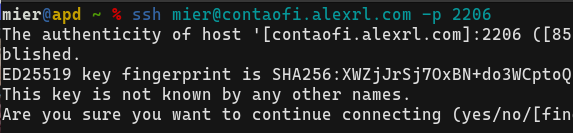
\includegraphics[width=\textwidth]{3/ssh1.png}
    \captionof{figure}{Fingerprint del servidor SSH}\label{fig:3/6}
\end{minipage}

\subsubsection{Ejercicio 4}
Para este ejercicio, en lugar de utilizar PuTTYgen, se utiliza el comando \Verb#ssh-keygen#
para generar la clave RSA{.}

\begin{minipage}{\linewidth}
    \centering
    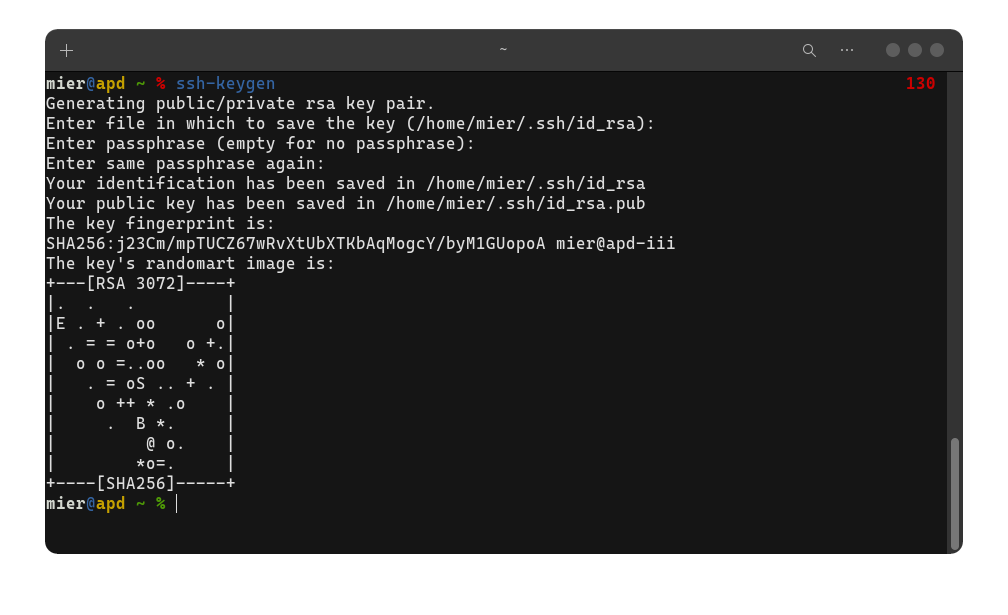
\includegraphics[width=\textwidth]{3/ssh2.png}
    \captionof{figure}{Generación de claves RSA}\label{fig:3/7}
\end{minipage}

El comando guarda automáticamente las claves en el directorio \Verb#~/.ssh# con los
nombres \Verb#id_rsa# y \Verb#id_rsa.pub#. Para poder utilizarlas, se copia la clave
pública al servidor remoto, en el fichero \Verb#~/.ssh/authorized_keys#.

\subsubsection{Ejercicio 5, 6}
Para utilizar las claves generadas en el ejercicio anterior, se ejecuta el comando
\Verb#ssh# junto con la opción \Verb#-i# para indicar la clave privada a utilizar.

\begin{minipage}{\linewidth}
    \centering
    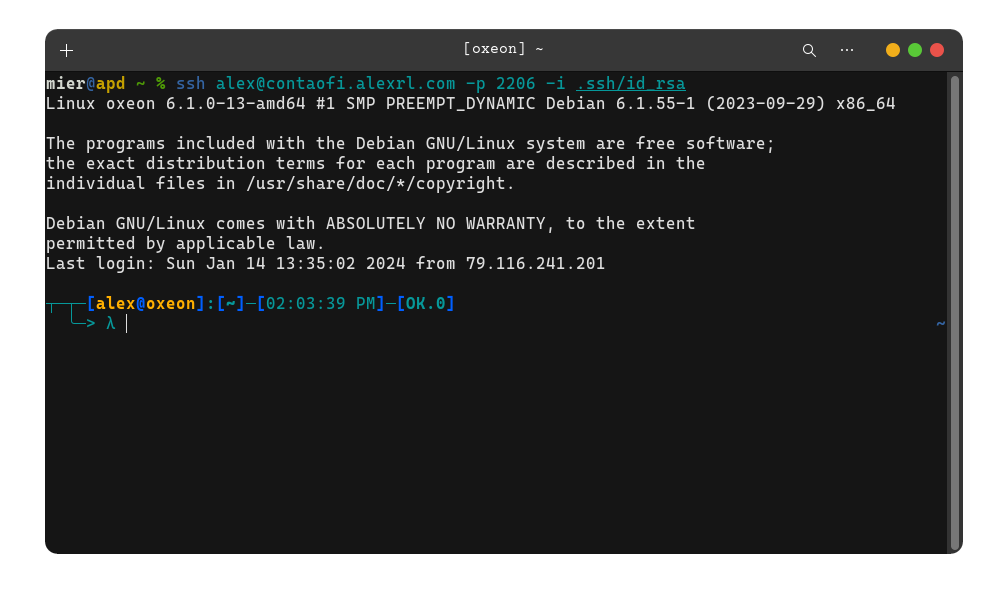
\includegraphics[width=\textwidth]{3/ssh3.png}
    \captionof{figure}{Conexión SSH con clave RSA}\label{fig:3/8}
\end{minipage}

\subsubsection{Ejercicio 7}
En lugar de \Verb#pageant#, se utiliza el comando \Verb#ssh-agent# para gestionar
las claves. Para añadir la clave privada al agente, se utiliza el comando
\Verb#ssh-add#. Para comprobar que la clave se ha añadido correctamente, se utiliza
el comando \Verb#ssh-add -l#.

\begin{minipage}{\linewidth}
    \centering
    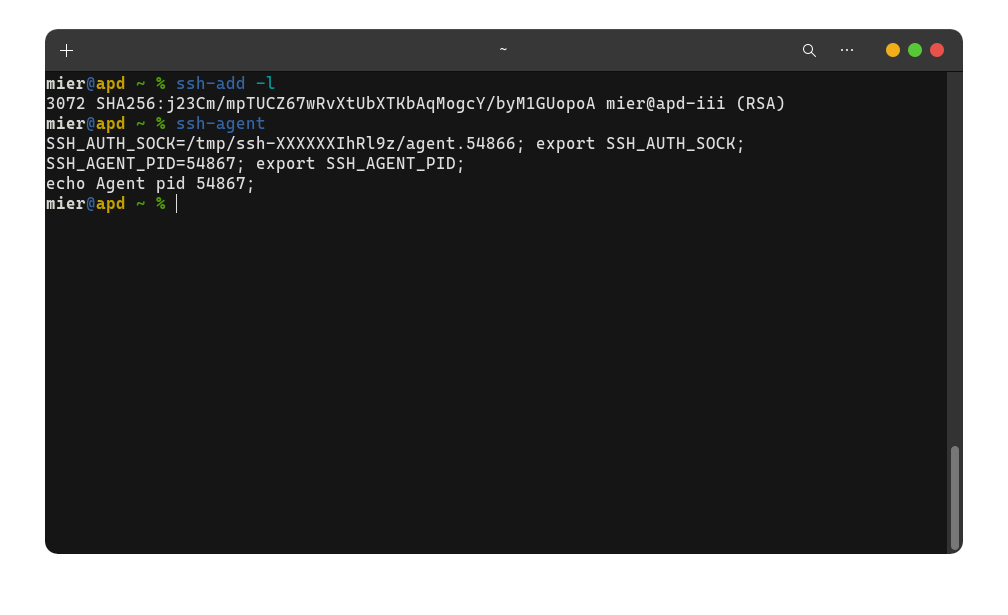
\includegraphics[width=\textwidth]{3/ssh4.png}
    \captionof{figure}{Gestión de claves con ssh-agent}\label{fig:3/9}
\end{minipage}

\begin{minipage}{\linewidth}
    \centering
    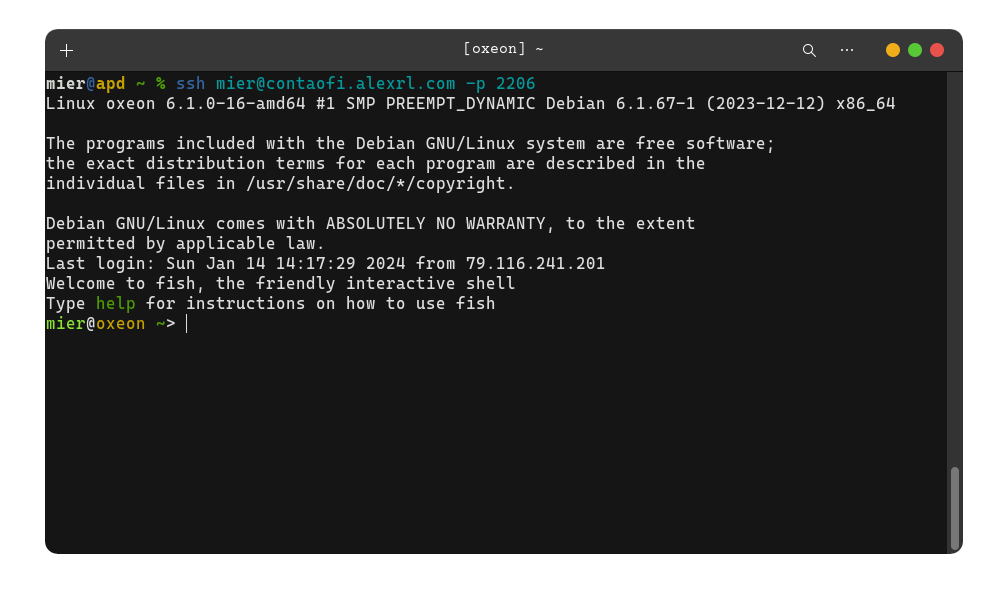
\includegraphics[width=\textwidth]{3/ssh5.png}
    \captionof{figure}{Demostración de autenticación mediante el agente}\label{fig:3/10}
\end{minipage}

\subsubsection{Ejercicio 8}
El ejercicio solicita que se modifique el programa \Verb#ssh_ejemplo_mal.py#
para que incluya la línea \Verb#client.set_missing_host_key_policy(paramiko.AutoAddPolicy())#
(resultando en el \Verb#ssh_ejemplo_inseguro.py#). Introducimos la línea en cuestión entre la
creación del cliente \Verb#paramiko# y la conexión con el servidor ssh para hacer que el cliente
acepte cualquier clave que le envíe el servidor.

Como dice el enunciado, la ejecución de esta ``solución'' resulta en un error.

\begin{minipage}{\linewidth}
    \centering
    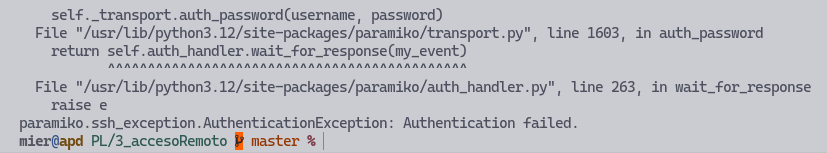
\includegraphics[width=\textwidth]{3/ssh6.png}
    \captionof{figure}{Error en la ejecución del ejemplo inseguro.}\label{fig:3/11}
\end{minipage}

La alternativa a esto es preguntarle al usuario directamente por la clave del servidor
y comprobar que es correcta antes de aceptarla.

\subsubsection{Ejercicio 9}
El ejercicio solicita que se modifique el programa \Verb#ssh_ejemplo_inseguro.py#
para que el cliente utilice la \Verb#WarningPolicy#.

Modificamos la política de la línea introducida en el ejercicio anterior y
obtenemos el fichero \Verb#ssh_ejemplo_inseguro2.py#. Este script sí que ejecuta
correctamente, pero muestra un mensaje de advertencia al usuario.

\begin{minipage}{\linewidth}
    \centering
    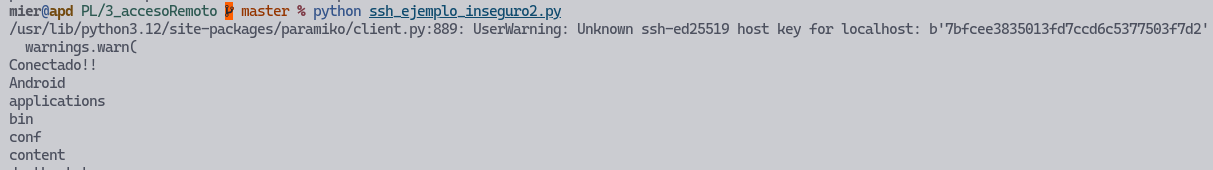
\includegraphics[width=\textwidth]{3/ssh7.png}
    \captionof{figure}{Ejecución del ejemplo inseguro 2.}\label{fig:3/12}
\end{minipage}

\subsubsection{Ejercicio 10}
El ejercicio solicita que se modifique el programa \Verb#ssh_ejemplo_inseguro2.py#,
eliminando la línea añadida previamente e insertando dos líneas nuevas para asegurar la conexión.

Para completar este ejercicio es necesario acceder al fichero \\
\Verb#/etc/ssh/ssh_host_ed25519_key.pub#, y añadir la clave pública del servidor,
que se pide por terminal al usuario.

\subsubsection{Ejercicio 11}

El ejercicio solicita que se modifique el programa \Verb#ssh_ejemplo_seguro.py#
para que sea posible conectarse al ordenador del compañero. Sigue la misma dinámica
de los ejercicios anteriores.

\section{Transferencia de archivos}
En esta sección se utilizan los protocolos \Verb#scp# y \Verb#sftp# para transferir
archivos entre máquinas remotas. Puesto que no se entra en muchos detalles en el
enunciado de la práctica, tampoco se comentan muchos detalles en esta memoria.

\subsubsection{Ejercicio 12}
Este ejercicio solicita que se utilice el programa \Verb#sftp# para conectarse a un
servidor remoto y listar los archivos que contiene.

\begin{minipage}{\linewidth}
    \centering
    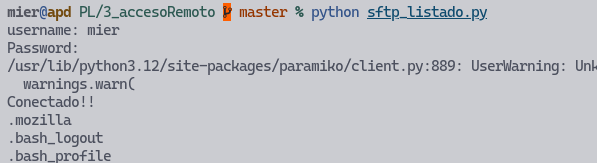
\includegraphics[width=\textwidth]{3/sftp1.png}
    \captionof{figure}{Listado de archivos con sftp}\label{fig:3/13}
\end{minipage}

\subsubsection{Ejercicio 13}
Este ejercicio solicita que se utilice el programa \Verb#sftp# para conectarse a un
servidor remoto y descargar todos los archivos (no directorios) del directorio \Verb#HOME#.

Se comenta el comando que descarga los ficheros para evitar tener que estar borrando y
descargando los ficheros cada vez que se ejecuta el script.

\begin{minipage}{\linewidth}
    \centering
    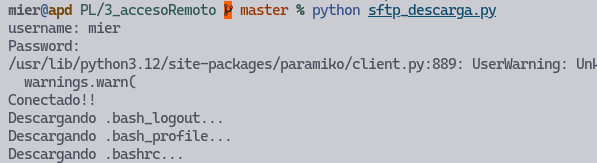
\includegraphics[width=\textwidth]{3/sftp2.png}
    \captionof{figure}{Descarga de archivos con sftp}\label{fig:3/14}
\end{minipage}

\chapter{Protocolos de DNS y correo electrónico}\label{chap:4}

\chapter{Contenido multimedia y streaming}\label{chap:5}
\section{Vídeo en la web}
\subsection{Ejercicio 1}
Una vez creado el \Verb#index.html#, se lanza la imagen de docker mediante el
siguiente comando:
\begin{verbatim}
docker run --rm -d --network pruebas --name nginx -p 80:80
    -v $(pwd)/html/video5/:/usr/share/nginx/html nginx
\end{verbatim}

Al acceder a \Verb#localhost:80#, se accede correctamente a la página web: \\
\begin{minipage}{\linewidth}
	\centering
	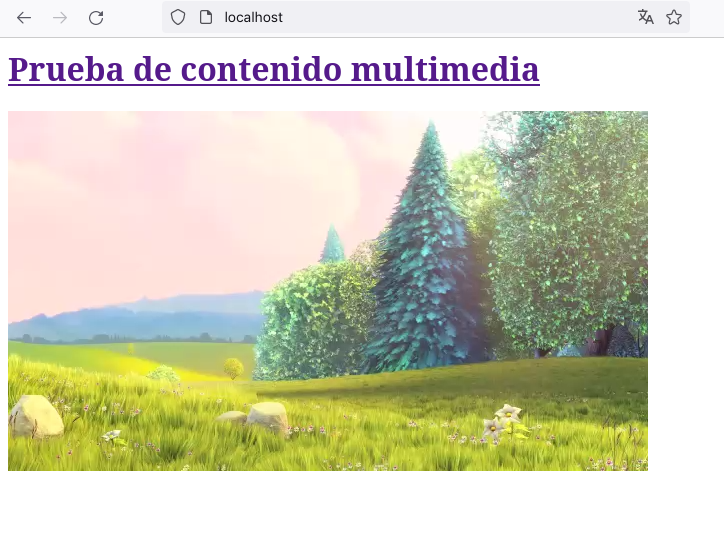
\includegraphics[width=0.8\textwidth]{5/1.png}
	\captionof{figure}{Página web con el vídeo}\label{fig:5/1}
\end{minipage}

Mediante las herramientas de desarrollador, se aprecia que se descargan fragmentos del vídeo
según se necesiten, incluyendo las cabeceras que especifican el rango de bytes a descargar: \\
\begin{minipage}{\linewidth}
	\centering
	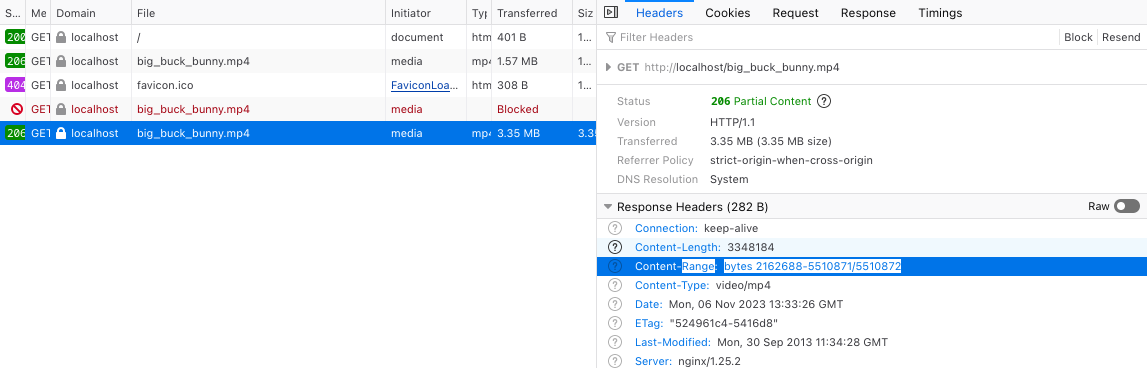
\includegraphics[width=0.8\textwidth]{5/2.png}
	\captionof{figure}{Cabeceras de la descarga del vídeo}\label{fig:5/2}
\end{minipage}

\subsubsection{Modifica ahora la página y utiliza como fuente otro vídeo}
En mi caso, Firefox en Linux admite los tres formatos disponibles (\Verb#mp4#, \Verb#webm# y \Verb#ogv#).
|TODO| revisar

\subsubsection{Modifica la página anterior para incluir todas las fuentes disponibles}
Este ejercicio no tiene más gracia que añadir las tres fuentes disponibles en la página web,
una detrás de otra junto con un mensaje de error en caso de que no se pueda reproducir el vídeo.

\begin{verbatim}
...
<source ... type="video/ogg;  codecs...">
<source ... type="video/mp4;  codecs...">
<source ... type="video/webm; codecs...">

<object type="application/x-shockwave-flash" ...>
	...
	<!-- Fallback final: -->
	<p>No se puede reproducir el video</p>
</object>
...
\end{verbatim}

\subsection{Ejercicio 2.~videojs}

\section{Servidor de streaming}

\Chapter{XMPP}{Mensajería}

\chapter{Servicios en móviles}\label{chap:7}
\section{Introducción al consumo de servicios desde móviles}

Esta sesión sirve de introducción al desarrollo de aplicaciones Android
utilizando Android Studio en Java.

En esta sesión se desarrolla una aplicación capaz de convertir euros
a dólares y viceversa.

Incialmente, se desarrolla un conversor simple que tiene el ratio de
conversión fijado en el código.
Posteriormente, se mejorará la aplicación utilizando una petición HTTP
que obtenga el ratio actualizado al momento.

\subsection{Converter simple}

Al crear el proyecto, seleccionamos el Android SDK Platform 33.

Posteriormente, creamos un dispositivo virtual que permita probar la
aplicación sin utilizar nuestro dispositivo físico.
Seleccionamos un Nexus 5X con Nougat (Android 7.0).

La interfaz de usuario consiste en dos campos de texto y dos botones.
Uno de los campos de texto contiene el valor en euros
y el otro la misma cantidad en dólares.
Al utilizar los botones se escribe en el otro campo de texto la cantidad
correspondiente en la moneda correspondiente.

Esto es, si se escribe el campo de texto de los euros
y se pulsa el botón de convertir a dólares,
se leerá la cantidad de euros del campo de texto de euros
y se escribirá la cantidad equivalente en dólares en el campo correspondiente.

La lógica de esta aplicación consiste en 3 funciones.

\begin{itemize}
    \item Función para convertir monedas en función de un ratio.
    \item Función para convertir de euros a dólares.
    \item Función para convertir de dólares a euros.
\end{itemize}

Por el momento se selecciona un valor fijo del ratio entre euros y dólares.

\subsection{Converter avanzado}

A continuación, se utilizará una API HTTP para obtener el ratio de euros a dólares.

Para acceder a esta API, se utilizará la libería Volley.
Para añadir Volley, utilizamos el manifiesto.

La API a utilizar (ExchangeRate) requiere que nos registremos y obtengamos un token
que nos permitirá realizar una cantidad fija de conversiones de forma gratuita.
Tras obtener dicho token, podemos introducirlo en la petición GET que realizamos con
Volley para obtener el ratio de conversión entre euros y dólares.

La petición de Volley no es instantánea, por lo que utilizamos una función de callback
que se ejecutará cuando llegue la respuesta a la petición de vuelta.
En esta función, extraemos de la respuesta el ratio de conversión y lo almacenamos
para poder utilizarlo en la función que convierte una moneda en otra.

Aquí se muestra un mensaje con el valor obtenido por la petición para el cambio de moneda:

\begin{minipage}{\linewidth}
	\centering
	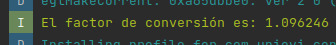
\includegraphics[width=\textwidth]{71/Conversion.jpg}
	\captionof{figure}{Ratio de EUR a USD}\label{fig:71/1}
\end{minipage}

A continuación, se muestra una captura de pantalla de la interfaz de usuario tras
haber realizado un cambio de euros a dólares:

\begin{minipage}{\linewidth}
	\centering
	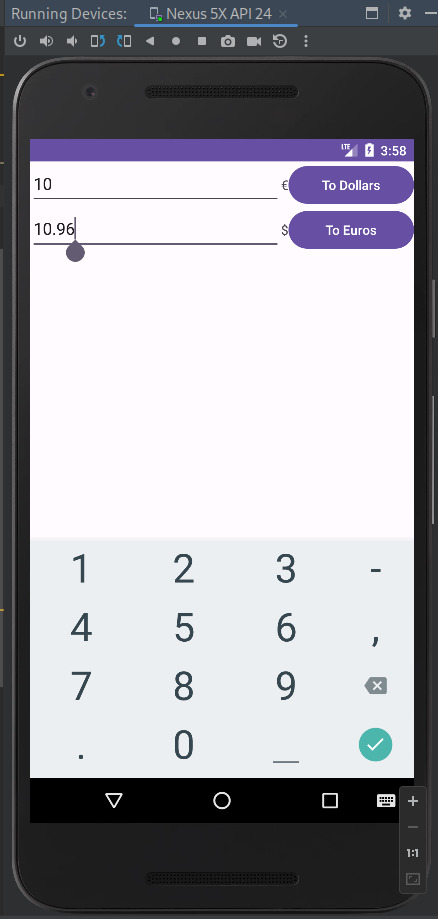
\includegraphics[width=0.4\textwidth]{71/App.jpg}
	\captionof{figure}{Aplicación}\label{fig:71/1}
\end{minipage}

\section{Integración de servicios sobre móviles}\label{sec:7/2}

\subsection{Pintar amigos en el mapa}

\subsection{Integración de serivcios web}

\subsection{Actualización de la posición en función del GPS}

\subsection{Servicios de notificaciones}


%% Esto incluirá la bibliografía correctamente en nuestro trabajo
\newpage{} % En una nueva página
\addcontentsline{toc}{chapter}{Bibliografía} % Añade la referencia al índice de contenido

\bibliographystyle{ieeetr} % Define el estilo de la bibliografía
\bibliography{biblio} % Indica el archivo que contiene la colección de citas

\nocite{template}

\end{document}
